\documentclass[12pt]{article}
\usepackage[hidelinks]{hyperref}
\usepackage[square,sort,comma,numbers]{natbib}
\usepackage{graphicx}
\title{Literature Survey}
\author{
    Andrew Mason\\
    \texttt{ajm188@case.edu}
    \and
    Jon Pfeil\\
    \texttt{jwp69@case.edu}
}
\date{December 8, 2014}
\begin{document}
\maketitle
\tableofcontents
\pagebreak

\section{Introduction and Software Verification}
Knowing that a software system fulfills a set of requirements correctly is an
important concern in industry, especially for mission-critical software
systems, such as the avionics software in an airplane, or the software in
medical devices. Approaches to software verification can be separated into
categories, dynamic approaches and static approaches.
\\

\noindent Dynamic approaches to software verification include unit testing,
integration and system testing, and acceptance testing. While these methods 
can identify bugs in the software and help improve software quality, alone they
cannot confirm that the system is bug free and that the system fulfills all of
its requirements. A requirement may not be excerised by the tests, and there
may be a bug that occurs only on a particular input which the test suite does
not include.
\\

\noindent We prefer instead the static methods of software verification, known
also as program analysis or formal verification. These techniques aim to
provide a formal proof that a system satisfies a specified property. Numerous
approaches to formal verification exist, and we briefly highlight a few of
them below.
\\

\noindent Model-based certification aims to provide formal proofs that an
abstract model, such as a formal computational model, representing the software
system has a particular property\cite{FormalSoftwareVerification}. In this
approach, a verifier uses a model-checking tool to explore the state space of
the program, searching for error states, states where a certain property of the
system does not hold. One issue with this approach is that the state space for
even trivial programs can grow quite large, but predicate abstraction can be 
used to systematically reduce the state space\cite{FormalSoftwareVerification}.
\\

\noindent Deductive software proving, also referred to as program proving, aims
to express the correctness of a program as a set of mathematical statements,
which are then discharged using a theorem prover
\cite{DeductiveSoftwareVerification}. To do this, a formal specification
language must be defined and integrated with the desired programming language.
Filliâtre claims that the best method for achieving this is to tighten a
specification language to a programming language within a dedicated program
logic, which mixes programs and logical statements, infusing program
contstructs with logical ones in a single language
\cite{DeductiveSoftwareVerification}.

\section{Specification Mining}
Formal software verification has the potential to replace testing as the
standard method of verifying program correctness. However, formal program
verifiers are limited in that they can only check specified properties.
Additionally, authors Lo and Khoo claim that the difficulty in formulating a
set of formal properties has contributed to the lack of widespread adoption in
industry\cite{Lo_softwarespecification}. To solve this issue, the technique of
specification mining aims to discover non-trivial properties or specifications
in a software system to later be used by a program verifier.
\\

\noindent Several approaches to specification mining are described in the
literature, the first of which is a machine learning approach outlined by
Ammons et al. Their mining approach is based on program execution traces rather
than static analysis of source code. Ammons et al argue that this approach is
superior since the traces will only contain the feasible paths of execution.
Additionally, basing the mining on program traces ensure that only correct
execution paths are mined, thus preventing buggy paths from polluting the
results of the mining\cite{Ammons:2002:MS:503272.503275}. Their miner extracts
abstract scenarios from traces annotated with information about flow
dependence, which are then fed into an automaton learner to learn the
specifications. The workflow of the miner looks like
\cite{Ammons:2002:MS:503272.503275}:\\
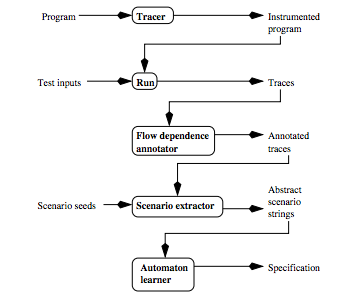
\includegraphics{machine_learning_miner_workflow.png}
\section{Code Clones}
\section{GSpan}
\subsection{Subgraph Isomorphism}
\subsection{Frequent Subgraph Mining}
\pagebreak
\bibliographystyle{acm}
\bibliography{lit_survey}
\end{document}
